\documentclass[11pt]{article}
\usepackage[utf8]{inputenc}
\usepackage[IL2]{fontenc}
\usepackage[czech]{babel}
\usepackage{wrapfig}
\usepackage[dvipdf]{graphicx}
\usepackage{color}
\usepackage{float}
\usepackage{amsmath}
\usepackage{amssymb}
\usepackage{hyperref}

\usepackage[total={15.5cm,23cm}, top=3cm, left=3cm, includefoot]{geometry}

\setlength\parindent{2em}

\usepackage{etoolbox}

\title{KIV/TI: Převod nedeterministického automatu na deterministický}
\author{Jaroslav Klaus, Vladimír Láznička}
\begin{document}
\begin{titlepage}

\includegraphics[width = 6cm]{logo_fav.jpg}
\begin{center}
\vfill
\textsc{\large KIV/TI - Teoretická informatika}\\
\textsc{\LARGE Převod nedeterministického automatu na deterministický}
\\[0.2cm]
\end{center}
\vfill
Jaroslav Klaus (A13B0347P), Vladimír Láznička (A13B0371P)
\\[0.2cm]
18. ledna 2015,  Plzeň
\end{titlepage}

\tableofcontents

\newpage

\section{Zadání}
Implementujte algoritmus pro převod nedeterministického konečného rozpoznávacího automatu (umožněte i existenci e-hran) na ekvivalentní deterministický automat. Navrhněte vhodný formát vstupních a výstupních dat.

Program odlaďte alespoň na 6 příkladech včetně příkladů prezentovaných na přednáškách a cvičeních.

Všechny testovací příklady uveďte v dokumentaci včetně ručního řešení.

\subsection{Formát vstupních a výstupních dat}
Jako formát vstupních a výstupních dat budeme volit textové soubory \texttt{*.TI} odpovídající definici nedeterministického konečného rozpoznávacího automatu (vstup) a deterministického konečného rozpoznávacího automatu (výstup) na stránce \url{http://home.zcu.cz/~vais/formaty.htm}. Cílem výstupu je pak možnost jej využít pro další zpracování (např. minimalizace) daného automatu dalším programem.

\newpage

\section{Analýza}
Řešení úlohy lze rozdělit do následujících celků - načtení dat ze vstupu a jejich zpracování do příslušné struktury, samotný převod automatu podle dané reprezentace na deterministický typ, uložení dat vzniklých z převodu do příslušné struktury a nakonec výpis výsledku na výstup.

\subsection{Zpracování vstupu}
Pro zpracování vstupu bude zapotřebí připravit si funkci nebo metodu, která provede \textbf{parsování vstupu na jednotlivé řetězce}, ze kterých se poté získají hodnoty důležité pro reprezentaci automatu a jeho následný převod. Formát vstupního souboru bude naprosto zásadní dodržet, neboť v opačném případě může dojít k chybnému převodu nebo také k němu nemusí dojít vůbec. Vstupní soubor nám udává \textbf{počet stavů automatu, velikost množiny vstupních symbolů, přechodovou tabulku automatu a nakonec výpis vstupních a výstupních stavů}. Tyto informace bude třeba uložit do struktury nebo objektu reprezentující daný automat.

Jako reprezentace chování automatu se pak využije zmíněná \textbf{přechodová tabulka}, která v sobě drží defacto všechny potřebné informace k jeho převodu na deterministický typ. Ostatní informace poslouží buď k vytvoření dalších celků (jako velikost polí na základě počtu stavů) nebo k závěrečné části převodu - určení vstupního stavu a výstupních stavů deterministického automatu. Samotný seznam stavů nebude ke způsobu zápisu vstupního souboru potřeba, neboť stavy vždy odpovídají \textbf{velkým písmenům a jsou řazené podle abecedy} (obdobně to platí pro množinu vstupních symbolů, nicméně tu nebudeme pro převodu automatu přímo potřebovat).

\subsection{Převod nedeterministického automatu na deterministický}
Převod bude probíhat pomocí \textbf{přechodové tabulky}, která se bude postupně upravovat, aby se z ní odstranily všechny nedeterminismy (více vstupních stavů, nejednoznačné přechody a přítomnost e-hran). To nám zajiští jistou inuitivnost a umožní snazší porovnání s ručním řešením, které bude rovněž prováděno na základě přechodové tabulky.

Při vytváření tabulky deterministického automatu se nejprve použije \textbf{první řádek tabulky z původního automatu}, který se bude procházet položku po položce, z nichž se vyberou ty stavy, které ještě nemáme zaznamenány (na počátku máme pouze jeden vstupní stav). Pokud bude položka obsahovat více stavů, tyto stavy se \textbf{spojí v jeden nový stav} a ten se zaznamená. Pro každý takto zaznamenaý stav se vytvoří další řádek, jeho položky budou obsahovat stavy, do kterých bychom se z něj dostali v daném nedeterministickém automatu pomocí příslušného vstupního znaku. Pokud byl nově vzniklý stav složen z více původních stavů, v položkách pro tento stav budou zaznamenány stavy, do kterých se lze daným znakem dostat ze všech těchto původních stavů. Takto se bude pokračovat, dokud nebudou nalezeny všechny nové stavy a pro ně vytvořeny příslušné položky.

V případě \textbf{více vstupních stavů} se tyto stavy na počátku převodu spojí v jeden a takto vzniklý stav se použije jako první zaznamenaný. Pokud bude nedeterministický automat obsahovat \textbf{e-hrany}, což je indikováno další položkou pro příslušný stav v původní přechodové tabulce \footnote{jejich počet pak o 1 přesahuje uvedenou velikost množiny vstupních znaků}, budeme vytvářet navíc tzv. tabulku \textbf{e-následníků}, která bude pro každý stav z původního automatu uvádět, do jakých dalších stavů se lze dostat prostřednictvím e-hrany (včetně jeho samého). Tyto stavy se pak sjednotí do jednoho nového, který bude mít vlastnosti všech v sobě obsažených stavů a \textbf{bude reprezentovat původní stav}, pro nějž se tito e-následníci zjišťovali.

Jakmile budeme mít vytvořenou přechodovu tabulku deterministického automatu, určíme pomocí \textbf{seznamu výstupních stavů} z nedeterministického automatu, jaké stavy budou výstupní v deterministickém automatu. Budou to ty, které v sobě obsahují nějaký výstupní stav z původního automatu. Jako stav vstupní se použije buď ten původní, pokud byl jeden, nebo stav vzniklý sjednocením několika původních stavů, pokud jich bylo více.

\subsection{Uložení parametrů deterministického automatu a vypsání výstupu}
Vzhledem k tomu, že z předchozí části již budeme mít všechny potřebné informace - \textbf{počet stavů, přechodovou tabulku, vstupní stav a výstupní stavy}, lze je jednoduše uložit do stejné struktury nebo objektu jako u nedeterministického automatu. Pak už jen stačí použít vhodnou funkci nebo metodu, která si tyto informace vezme a zapíše je do souboru v daném formátu (v zásadě bude fungovat přesně opačně než funkce pro načtení dat ze souboru). 

\newpage

\section{Implementace programu}
K implementaci programu jsme se rozhodli použít jazyk \textbf{Java}, který je jednak výhodný svým objektovým přístupem a také obsahuje několik knihovních tříd umožňující používání různých struktur jako třeba seznamy, aniž bychom je museli sami implementovat. Nevýhodou je pak samozřejmě pomalejší běh než např. při použití jazyka \textbf{C}, ale pro náš případ není vysoká rychlost zpracování až tak důležitá.

\subsection{Objekt Automaton}
Tento objekt slouží k \textbf{uchování informací o automatu ve svých atributech}. Těmito atributy jsou:

\begin{itemize}
\item \texttt{String automatonType} - řetězec obsahující zkratku typu automatu
\item \texttt{int statusCnt} - počet stavů automatu 
\item \texttt{int inputCnt} - velikost množiny vstupních znaků
\item \texttt{String[][] automatonTable} - pole uchovávající přechodovu tabulku automatu, každý řádek přísluší jednomu stavu (A... Z) a každý sloupec jednomu vstupnímu znaku (a... z).
\item \texttt{ArrayList<String> inputStatuses} - seznam se vstupními stavy automatu
\item \texttt{ArrayList<String> outputStatuses} - seznam s výstupními stavy automatu
\end{itemize}

Dále má samozřejmě metody pro ukládání a vracení těchto atributů, kde je to třeba. Konstruktor pak jako parametry přijímá \textbf{zkratku automatu, počet stavů a počet vstupních znaků}.

\subsection{Načtení souboru a uložení dat}
Načtení souboru je řešeno pomocí metody \texttt{static createAutomatonFromFile(String filePath)}, která přebírá jako parametr řetězec s cestou ke vstupnímu souboru a je obsažena ve třídě \texttt{Input\_Output}. Metoda používá ke čtení souboru knihovní třídu \texttt{BufferedReader}, zejména její metodu \texttt{readLine()}, pomocí které získa řetězec představující obsah aktuálně načítaného řádku. Ten je pak rozdělen buď ručně nebo pomocí metody \texttt{split()}, přičemž jako dělící znak je použita mezera. Nejprve se načte typ automatu, počet stavů a počet vstupních znaků a tyto hodnoty se poté použijí k vytvoření objektu \texttt{Automaton}. Následně se načte přechodová tabulka a postupně uloží do \textbf{dvourozměrného pole řetězců}, které se pak objektu předá. Nakonec se načtou vstupní a výstupní stavy do příslušných seznamů a rovněž se předají objektu.

\subsection{Algoritmus převodu}
Samotný převod je implementován ve třídě \texttt{Convert} a v její hlavní metodě \texttt{public static Automaton nkaToDka(Automaton nka)}, která jako parametr přebírá nedeterministický konečný automat (dále NKA), který se načetl ze vstupního souboru. Nejprve se vytvoří tabulka e-následníků pomocí metody \texttt{private static void createETable(String[][] nkaTable, int inputCount, String[] eTable)}. Jako první stav deterministického konečného automatu (dále DKA) se použije sjednocení vstupních stavů NKA a jejich e-následníků. Tento první stav se vloží do fronty \texttt{statuses}. Dokud bude ve frontě \texttt{statuses} nějaká položka, vybere se první položka a do nové řádky přechodové tabulka DKA se zapisují nové stavy, do kterých se dostaneme příslušným vstupním symbolem. Zjišťování těchto stavů probíhá tak, že sjednotíme stavy, do kterých se z původních stavů NKA dostaneme pomocí vstupního symbolu, a přidáme jejich e-následníky. Pokud takto nově vzniklý stav není ve frontě \texttt{statuses}, tak jej do ní přidám a pokračuji pro další sloupec tabulky (další vstupní symbol). Toto opakuji, dokud mi vznikají nové stavy v přechodové tabulce DKA, respektive dokud není fronta \texttt{statuses} prázdná.

\subsection{Uložení výsledného automatu a výpis na výstup}
Výsledný deterministický automat je vytvořen na konci metody pro převod. Nejprve se vytvoří objekt tohoto automatu, přičemž jako parametry jsou použity řetězec "DKAR" (deterministický konečný automat rozpoznávací - dle požadovaného formátu souboru), velikost seznamu s vytvořenými stavy a počet vstupních znaků z původního automatu (ten se převodem nijak nemění). Poté se uloží pomocí metody \texttt{static void setOuputStatusesToDka(Automaton nka, Automaton dka, LinkedList<String> statuses)} seznam výstupních stavů automatu postupem víceméně popsaným v analýze. V metodě také dojde k přejmenování stavů tak, aby vyhovovaly formátu souboru, který bude výstupem. Přejmenování probíhá procházením vytvořených výstupních stavů, které mohou být v tu chvíli označené jako složení původních stavů, přičemž se tyto stavy porovnávají se seznamem všech nově vytvořených stavů a jakmile dojde ke shodě, složený stav se přejmenuje podle formule \texttt{'A'+ index stavu v seznamu vytvořených stavů}. K podobnému přejmenování dojde i ve vytvořené přechodové tabulce v metodě \texttt{static void renameStatuses(String[][] dkaTable, LinkedList<String> statuses)}. Nakonec se tabulka předá objektu automatu a tytvoří se list s jednim stavem \texttt{"A"}, který je uložen jako vstupní (prezentuje množinu původní vstupních stavů).

Objekt se pak použije k výpisu informací do výstupního souboru pomocí metody \texttt{static void writeAutomatonToFile(Automaton a, String filepath)} ze třídy \texttt{Input\_Output}. V zásadě funguje opačně než metoda pro získání dat ze souboru. Postupně skládá informace získané z objektu automatu do řetězců, představující jednotlivé řádky (podle požadovaného formátu) a ty pomocí metody \texttt{write(<retezec>)} z knihovní třídy \texttt{BufferedWriter} zapisuje do zadaného souboru. 
-doplnit-

\newpage

\section{Uživatelská dokumentace}

Pro spuštění programu je zapotřebí mít na počítači nainstalované prostředí \textbf{Java Runtime Environment 1.8 nebo novější} (na této verzi bylo vykonána kompilace programu). Spuštění lze pak provést z příkazové řádky, odkud se spouští JAR archiv aplikace pojmenovaný \textbf{NKAR\_to\_DKAR\_App.jar}.

Příkaz ke spuštění je následující: \texttt{java -jar NKAR\_to\_DKAR\_App.jar <vstupni\_soubor> <vystupni\_soubor>}

Vstupní soubor musí obsahovat informace ve specifickém formátu zobrazeném na stránkách zmíněných v části \textbf{Zadání}. Výstupní soubor pak označuje soubor, do kterého se v obdobném formátu zapíše převedený automat. Pokud je toto splněno, proběhne převod a vytvoří se výstupní soubor s převedeným automatem (při každém dalším použití programu se soubor přepíše, pokud použijeme stejný název).

\begin{figure}[htbp]
\centering
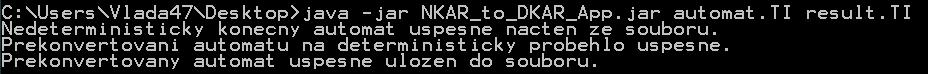
\includegraphics[width = 15cm]{success.jpg}
\begin{center}
\caption{Korektní spuštění programu}
\end{center}
\end{figure}

Pokud nedodržíme uvedené podmínky, program skončí chybovým hlášením. Stejně tak, pokud dojde během zpracování vstupu nebo převodu k nějaké vyjímce.

\begin{figure}[htbp]
\centering
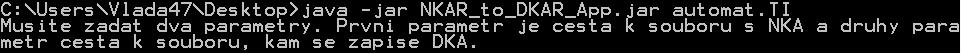
\includegraphics[width = 15cm]{fail.jpg}
\begin{center}
\caption{Chyba při zadání příliš málo vstupní parametrů}
\end{center}
\end{figure}

\newpage

\section{Ověření správnosti převodu}

-doplnit-

\newpage

\section{Závěr}

-doplnit-

\end{document}